\documentclass[a4paper, 12pt]{article}
\usepackage[UTF8]{ctex}
\usepackage{geometry}
\usepackage{graphicx}
\usepackage{float}
\usepackage{hyperref}
\usepackage{tcolorbox}
\tcbuselibrary{most}

% 设置页边距
\geometry{a4paper, left=2.5cm, right=2.5cm, top=2.5cm, bottom=2.5cm}

% 简化实例方框样式
\tcbset{instancestyle/.style={
    enhanced,
    sharp corners,
    colback=white,
    colframe=black!70!white,
    boxrule=0.8pt,
    left=6pt,
    right=6pt,
    top=6pt,
    bottom=6pt,
    boxsep=2pt,
    arc=2pt
}}

\begin{document}

\title{\huge{系统开发工具基础实验报告2}}
\author{姓名:\underline{刘浩洋} \\ 
        学号:\underline{24040021022} \\ 
        班级:\underline{软件工程}}
\date{实验日期:\underline{2025年9月5日}}
\maketitle

\section*{一、实验目的}
\begin{enumerate}
    \item 掌握Linux系统中Shell的基本命令,包括文件、目录和路径操作;
    \item 熟悉Shell脚本编程基础,包括变量、条件判断、循环等结构;
    \item 掌握Vim文本编辑器的基本使用方法;
    \item 能够独立编写并运行简单的Shell脚本;
    \item 培养在虚拟机环境下使用Ubuntu进行系统开发工具实践的能力。
\end{enumerate}

\section*{二、实验环境}
\begin{itemize}
    \item 操作系统:Windows 11
    \item 虚拟化平台:VMware Workstation Pro 17
    \item 虚拟机系统:Ubuntu 24.04.3 LTS(64位)
    \item Shell环境:Bash
    \item 编辑器:Vim
\end{itemize}

\section*{三、练习内容}
本次实验主要包括:
\begin{itemize}
    \item 文件与目录的创建、复制、移动、删除;
    \item 绝对路径与相对路径的使用;
    \item Shell脚本中变量、条件判断、循环的使用;
    \item 使用Vim编辑脚本文件;
    \item 编写并运行综合Shell脚本。
\end{itemize}

\section*{四、20个实例(shell与vim)}

\begin{tcolorbox}[instancestyle, title=实例1:创建实验目录结构]
使用 mkdir 命令可以创建多级目录结构,
便于组织和管理实验相关文件。
该命令支持 -p 参数,可避免目录已存在时报错。

\texttt{mkdir -p ~/lab1/\{scripts,data,docs\}} \\
\texttt{cd ~/lab1} \\
\texttt{touch data/file1.txt data/file2.txt} \\
\texttt{ls} \\
\texttt{tree} \\
\texttt{pwd}
\end{tcolorbox}

\begin{tcolorbox}[instancestyle, title=实例2:文件复制与重命名]
cp 命令用于复制文件或目录,
mv 命令用于移动或重命名文件。
结合通配符 * 可批量操作多个文件。

\texttt{cp data/file1.txt scripts/} \\
\texttt{mv scripts/file1.txt scripts/test1.bak} \\
\texttt{cp data/*.txt scripts/} \\
\texttt{ls scripts/} \\
\texttt{rm data/file1.txt} \\
\texttt{ls data/}
\end{tcolorbox}

\begin{tcolorbox}[instancestyle, title=实例3:切换目录与路径使用]
Linux 中路径分为绝对路径和相对路径。
cd 命令用于切换当前工作目录。
使用 .. 可返回上级目录,~ 代表家目录。

\texttt{echo "当前目录:\$(pwd)"} \\
\texttt{cd /home/\$(whoami)/lab1/docs} \\
\texttt{cd ..} \\
\texttt{cd scripts} \\
\texttt{cd ~} \\
\texttt{cd -}
\end{tcolorbox}

\begin{tcolorbox}[instancestyle, title=实例4:查看与修改文件权限]
Linux 文件具有读、写、执行三种权限。
chmod 命令用于修改文件权限,
可使用符号模式(如 +x)或数字模式(如 755)。

\texttt{ls -l scripts/} \\
\texttt{chmod +x scripts/test1.bak} \\
\texttt{chmod 644 scripts/test1.bak} \\
\texttt{chmod -R 755 scripts/} \\
\texttt{ls -l scripts/} \\
\texttt{./scripts/test1.bak}
\end{tcolorbox}

\begin{tcolorbox}[instancestyle, title=实例5:编写第一个Shell脚本]
Shell 脚本以 \#!/bin/bash 开头,
表示使用 Bash 解释器执行。
echo 命令用于输出文本信息,
\$(date) 可嵌入当前系统时间。

\texttt{\#!/bin/bash} \\
\texttt{echo "欢迎使用Shell脚本!"} \\
\texttt{echo "当前时间:\$(date)"} \\
\texttt{echo "实验环境:Ubuntu 24.04"} \\
\texttt{echo "Shell版本:\$(bash --version | head -1)"} \\
\texttt{echo "当前用户:\$(whoami)"} \\
\texttt{echo "脚本执行完毕"}
\end{tcolorbox}

\begin{tcolorbox}[instancestyle, title=实例6:Shell变量定义与使用]
Shell 中变量无需声明即可使用,
变量名区分大小写,赋值时等号两侧不能有空格。
使用 \$变量名 可引用变量值,
变量可存储字符串、数字或命令结果。

\texttt{\#!/bin/bash} \\
\texttt{name="刘浩洋"} \\
\texttt{year=2025} \\
\texttt{school="软件工程"} \\
\texttt{echo "姓名:\$name"} \\
\texttt{echo "年份:\$year"} \\
\texttt{echo "学院:\$school"}
\end{tcolorbox}

\begin{tcolorbox}[instancestyle, title=实例7:使用read读取用户输入]
read 命令用于从标准输入读取一行内容,
并赋值给指定变量。
可配合 echo 提示用户输入,
实现交互式脚本功能。

\texttt{\#!/bin/bash} \\
\texttt{echo "请输入姓名:"} \\
\texttt{read name} \\
\texttt{echo "请输入学号:"} \\
\texttt{read student_id} \\
\texttt{echo "欢迎你,\$name(学号:\$student_id)!"} \\
\texttt{echo "开始实验..."}
\end{tcolorbox}

\begin{tcolorbox}[instancestyle, title=实例8:Shell数组操作]
Shell 支持一维数组,使用括号定义。
\$\{array[@]\} 表示数组所有元素,
可通过 for 循环遍历数组内容,
实现批量处理数据。

\texttt{\#!/bin/bash} \\
\texttt{fruits=("苹果" "香蕉" "橙子" "葡萄")} \\
\texttt{echo "水果列表:\$\{fruits[@]\}"} \\
\texttt{for f in "\$\{fruits[@]\}"; do} \\
\texttt{  echo " - \$f"} \\
\texttt{done} \\
\texttt{echo "共 \${#fruits[@]} 种水果"}
\end{tcolorbox}

\begin{tcolorbox}[instancestyle, title=实例9:if条件判断(数字)]
if 语句用于根据条件执行不同分支。
[ ] 内使用 -gt、-lt、-eq 等比较数字。
elif 表示否则如果,fi 表示 if 结束。

\texttt{\#!/bin/bash} \\
\texttt{read num} \\
\texttt{if [ \$num -gt 0 ]; then} \\
\texttt{  echo "\$num 是正数"} \\
\texttt{elif [ \$num -lt 0 ]; then} \\
\texttt{  echo "\$num 是负数"} \\
\texttt{else} \\
\texttt{  echo "\$num 是零"} \\
\texttt{fi}
\end{tcolorbox}

\begin{tcolorbox}[instancestyle, title=实例10:case多分支选择]
case 语句适用于多条件匹配场景。
每个分支以 ) 结尾,;; 表示结束。
* 表示默认匹配,esac 表示结束。

\texttt{\#!/bin/bash} \\
\texttt{echo "请选择功能:1) 日期  2) 磁盘  3) 内存"} \\
\texttt{read choice} \\
\texttt{case \$choice in} \\
\texttt{  1) echo "当前时间:"; date ;;} \\
\texttt{  2) echo "磁盘使用:"; df -h ;;} \\
\texttt{  3) echo "内存状态:"; free -h ;;} \\
\texttt{  *) echo "无效选择" ;;} \\
\texttt{esac}
\end{tcolorbox}

\begin{tcolorbox}[instancestyle, title=实例11:for循环遍历文件]
for 循环可用于遍历列表或文件。
使用通配符 *.sh 可匹配所有 Shell 脚本。
basename 命令提取文件名部分,
便于格式化输出。

\texttt{\#!/bin/bash} \\
\texttt{for file in scripts/*.sh; do} \\
\texttt{  if [ -f "\$file" ]; then} \\
\texttt{    echo "发现脚本:\$(basename \$file)"} \\
\texttt{    echo "  路径:\$file"} \\
\texttt{    echo "  大小:\$(du -h "\$file" | cut -f1)"} \\
\texttt{  fi} \\
\texttt{done}
\end{tcolorbox}

\begin{tcolorbox}[instancestyle, title=实例12:while循环计数]
while 循环在条件为真时持续执行。
常用于计数、监控或等待操作。
使用 sleep 可控制循环间隔时间。

\texttt{\#!/bin/bash} \\
\texttt{count=5} \\
\texttt{while [ \$count -gt 0 ]; do} \\
\texttt{  echo "\$count..."} \\
\texttt{  sleep 1} \\
\texttt{  count=\$((count - 1))} \\
\texttt{done} \\
\texttt{echo "倒计时结束!"}
\end{tcolorbox}

\begin{tcolorbox}[instancestyle, title=实例13:until循环使用]
until 循环在条件为假时持续执行,
当条件变为真时停止。
与 while 逻辑相反,适用于倒数等场景。

\texttt{\#!/bin/bash} \\
\texttt{num=10} \\
\texttt{until [ \$num -lt 1 ]; do} \\
\texttt{  echo "倒数:\$num"} \\
\texttt{  num=\$((num - 1))} \\
\texttt{  sleep 0.5} \\
\texttt{done} \\
\texttt{echo "发射!"}
\end{tcolorbox}

\begin{tcolorbox}[instancestyle, title=实例14:函数定义与调用]
函数用于封装可重复使用的代码块。
定义格式为 函数名() \{ ... \}。
使用 \$1、\$2 等引用传入参数。

\texttt{\#!/bin/bash} \\
\texttt{greet() \{} \\
\texttt{  echo "你好,\$1"} \\
\texttt{  echo "欢迎来到 \$2"} \\
\texttt{  echo "当前时间:\$(date +"\%H:\%M:\%S")"} \\
\texttt{\}} \\
\texttt{greet "张三" "Shell 实验"} \\
\texttt{greet "李四" "Linux 世界"}
\end{tcolorbox}

\begin{tcolorbox}[instancestyle, title=实例15:Vim的三种基本模式]
Vim 编辑器分为三种基本模式:命令模式、插入模式和底线命令模式。
启动 Vim 后默认进入命令模式,此时按键被视为命令而非输入。
按 i、a、o 等键可进入插入模式进行文本编辑。
按 : 进入底线命令模式可执行保存、退出等操作。

\texttt{vim test.txt} \\
\texttt{--- 启动后为命令模式 ---} \\
\texttt{i} \\
\texttt{输入一些文本内容...} \\
\texttt{Esc} \\
\texttt{:} \\
\texttt{:wq}
\end{tcolorbox}

\begin{tcolorbox}[instancestyle, title=实例16:进入与退出插入模式]
在命令模式下,按 i 在光标当前位置进入插入模式。
按 a 在光标后一个字符处开始输入。
按 o 在当前行下方插入新行并进入插入模式。
按 Esc 可随时返回命令模式。

\texttt{vim edit.txt} \\
\texttt{i} \\
\texttt{这是第一行文本。} \\
\texttt{a} \\
\texttt{继续在同一行输入。} \\
\texttt{o} \\
\texttt{这是新插入的一行。} \\
\texttt{Esc}
\end{tcolorbox}

\begin{tcolorbox}[instancestyle, title=实例17:替换模式与文本覆盖]
Vim 支持两种替换方式:单字符替换和连续替换。
按 r 可替换光标所在的一个字符,无需进入插入模式。
按 R 进入连续替换模式,后续输入将逐个覆盖原有字符。
此模式适合修改固定长度的文本内容。

\texttt{vim replace.txt} \\
\texttt{i} \\
\texttt{hello world} \\
\texttt{Esc} \\
\texttt{f w} \\
\texttt{r W} \\
\texttt{0} \\
\texttt{R} \\
\texttt{HELLO} \\
\texttt{Esc}
\end{tcolorbox}

\begin{tcolorbox}[instancestyle, title=实例18:保存与退出操作]
在底线命令模式中,:w 用于保存文件。
:q 用于退出,若已修改则需加 ! 强制退出。
:wq 或 ZZ 可保存并退出。
:q! 可放弃修改并强制退出。

\texttt{vim save.txt} \\
\texttt{i} \\
\texttt{这是一段测试文本。} \\
\texttt{Esc} \\
\texttt{:w} \\
\texttt{:q} \\
\texttt{--- 若未保存可 ---} \\
\texttt{:wq} \\
\texttt{:q!}
\end{tcolorbox}

\begin{tcolorbox}[instancestyle, title=实例19:光标移动与文本操作]
Vim 提供丰富的光标移动快捷键。
h、j、k、l 分别代表左、下、上、右。
0 移动到行首,$ 移动到行尾。
dd 删除整行,yy 复制,p 粘贴,u 撤销。

\texttt{vim move.txt} \\
\texttt{i} \\
\texttt{第一行} \\
\texttt{第二行} \\
\texttt{第三行} \\
\texttt{Esc} \\
\texttt{2G} \\
\texttt{dd} \\
\texttt{G} \\
\texttt{O} \\
\texttt{新行} \\
\texttt{yykP}
\end{tcolorbox}
\newpage
\begin{tcolorbox}[instancestyle, title=实例20:查找与全局替换]
在命令模式下,/keyword 可向下搜索文本。
?keyword 向上搜索,n 跳转下一个,N 跳转上一个。
在底线命令模式中,:\%s/old/new/g 可全局替换。
加 c 可确认每次替换。

\texttt{vim search.txt} \\
\texttt{i} \\
\texttt{apple banana apple} \\
\texttt{apple orange apple} \\
\texttt{Esc} \\
\texttt{/apple} \\
\texttt{n} \\
\texttt{N} \\
\texttt{:\%s/apple/fruit/g} \\
\texttt{:\%s/banana/mango/} \\
\texttt{:wq}
\end{tcolorbox}

\begin{figure}[htbp]
    \centering
    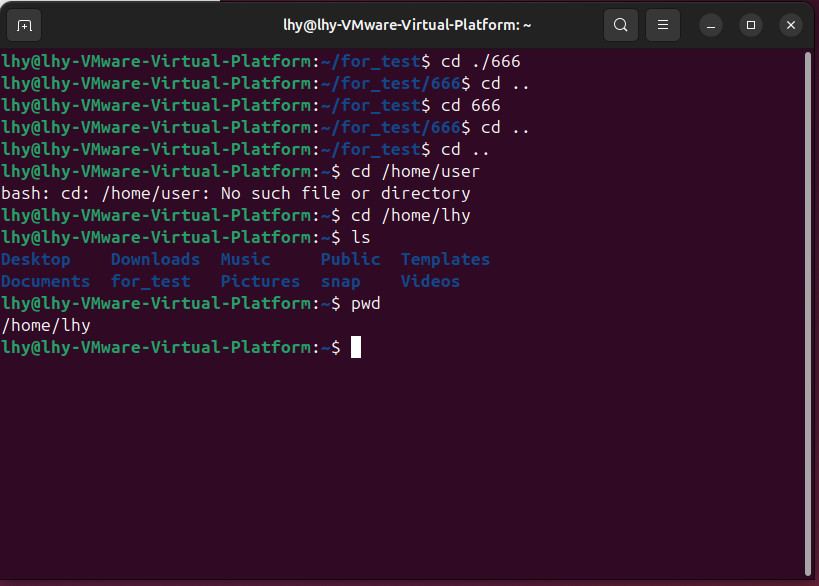
\includegraphics[width=0.8\textwidth]{lec2 (1).png}
    \caption{lec2 (1)}
    \label{fig:lec2-1}
\end{figure}

\begin{figure}[htbp]
    \centering
    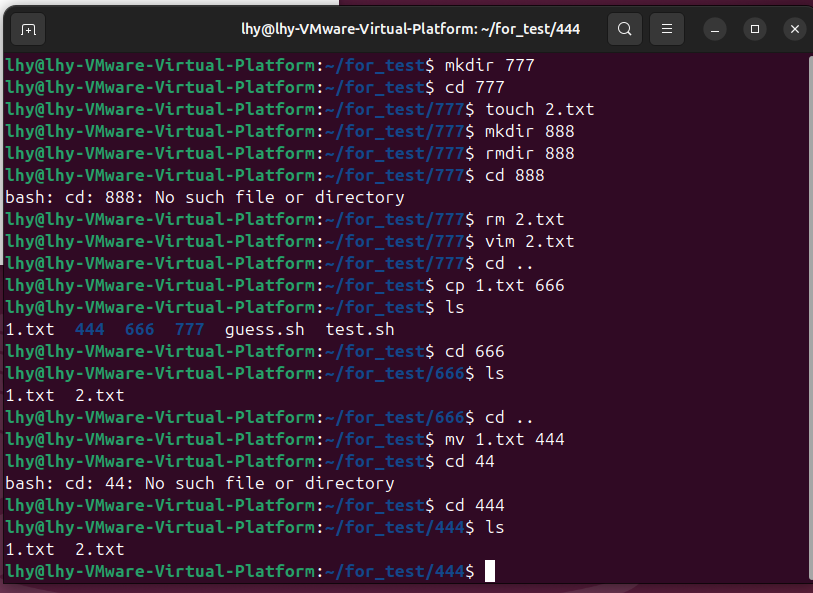
\includegraphics[width=0.8\textwidth]{lec2 (2).png}
    \caption{lec2 (2)}
    \label{fig:lec2-2}
\end{figure}

\begin{figure}[htbp]
    \centering
    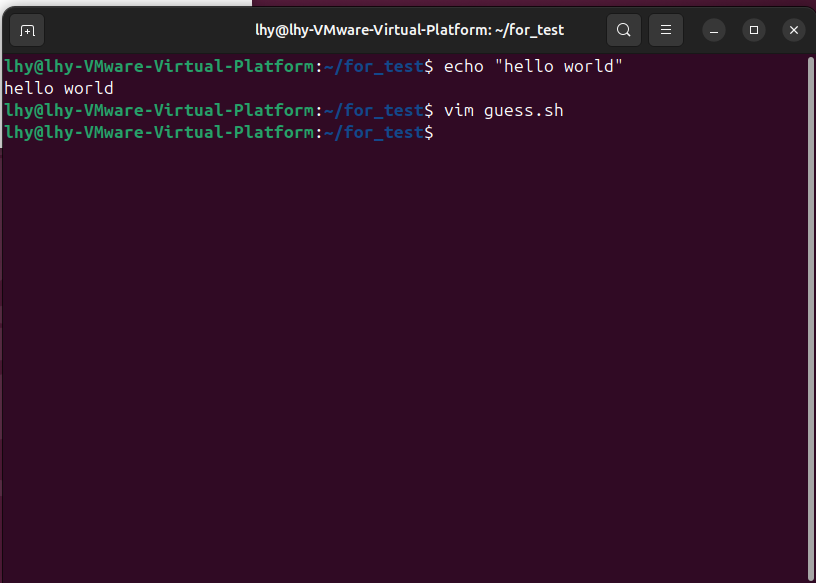
\includegraphics[width=0.8\textwidth]{lec2 (3).png}
    \caption{lec2 (3)}
    \label{fig:lec2-3}
\end{figure}

\begin{figure}[htbp]
    \centering
    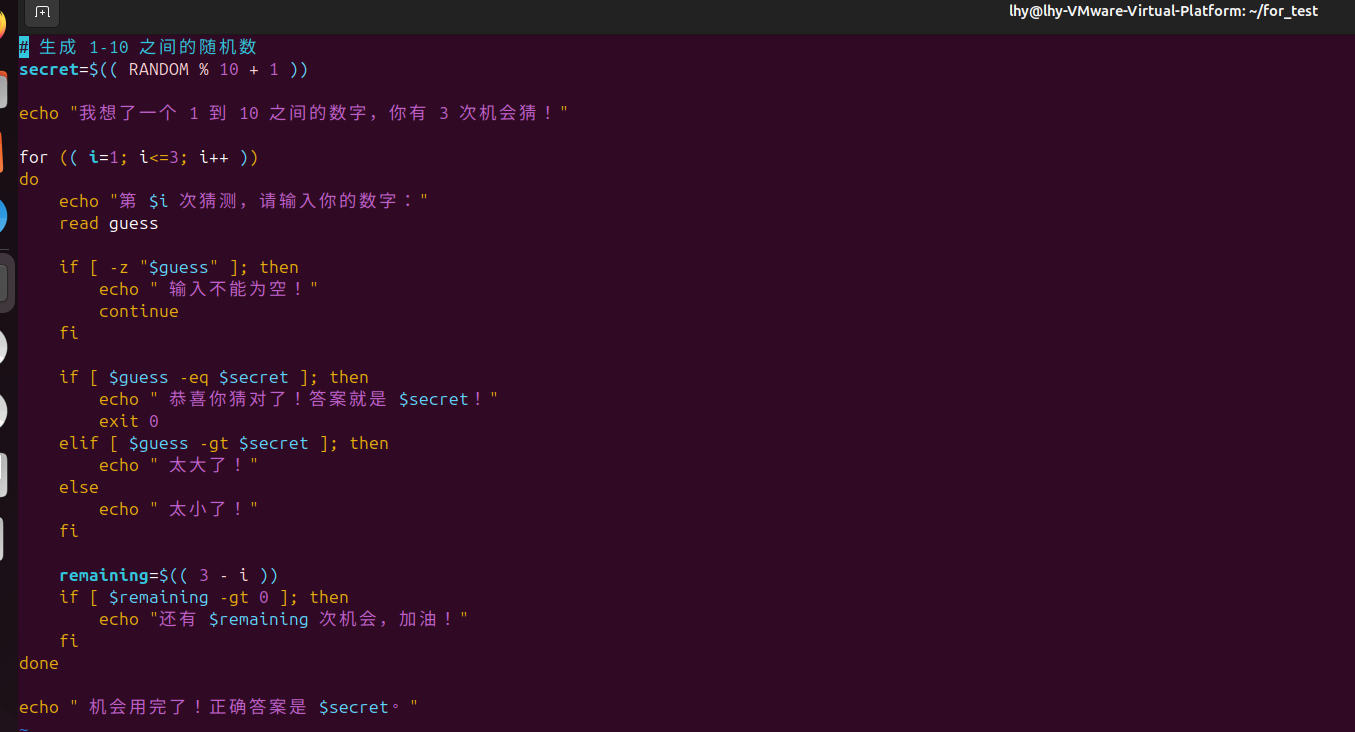
\includegraphics[width=0.8\textwidth]{lec2 (4).png}
    \caption{lec2 (4)}
    \label{fig:lec2-4}
\end{figure}

\begin{figure}[htbp]
    \centering
    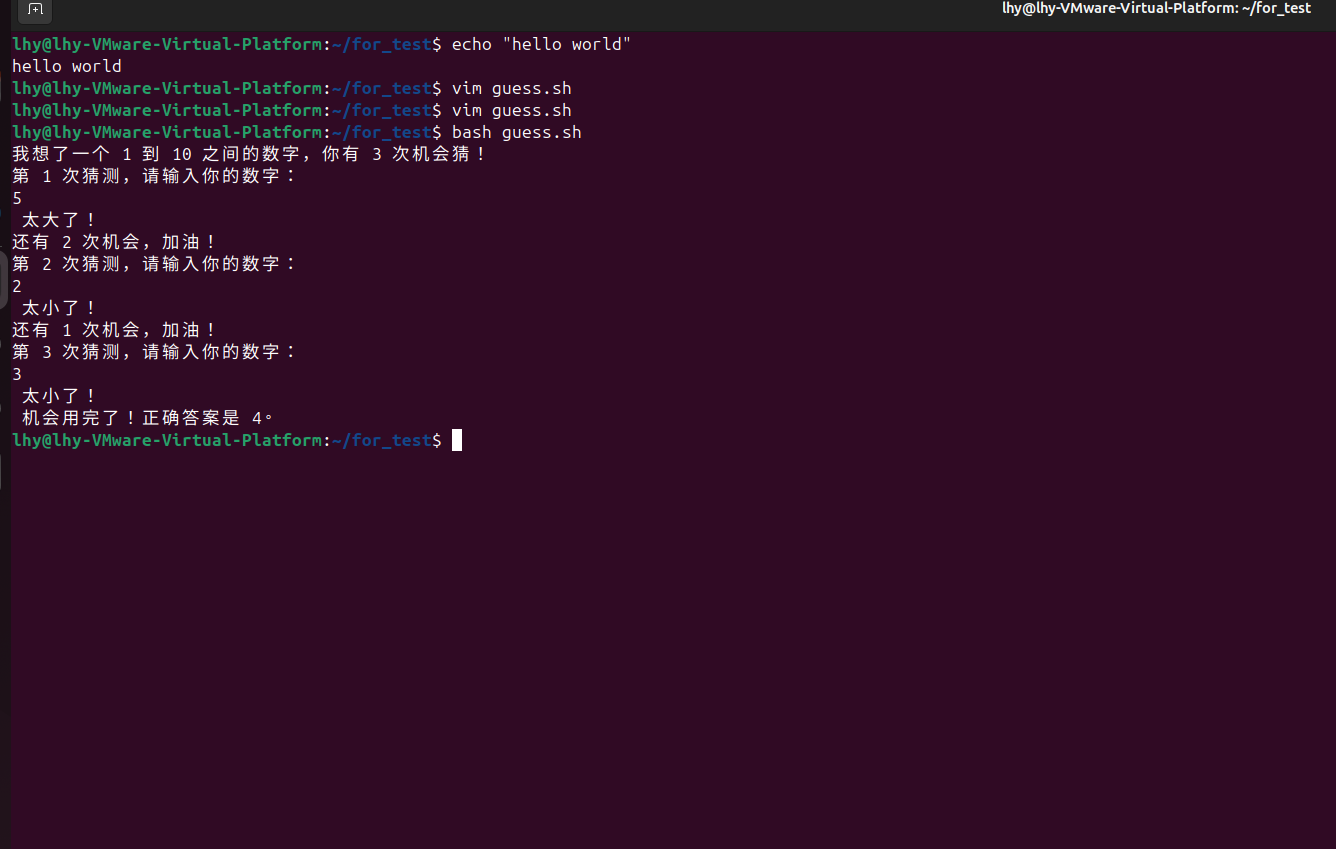
\includegraphics[width=0.8\textwidth]{lec2 (5).png}
    \caption{lec2 (5)}
    \label{fig:lec2-5}
\end{figure}

\begin{figure}[htbp]
    \centering
    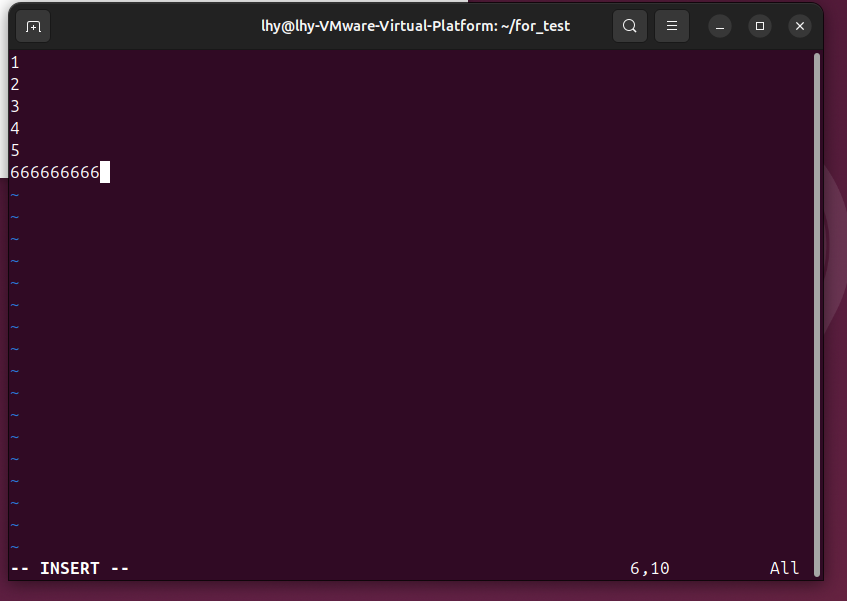
\includegraphics[width=0.8\textwidth]{lec2 (6).png}
    \caption{lec2 (6)}
    \label{fig:lec2-6}
\end{figure}

\begin{figure}[htbp]
    \centering
    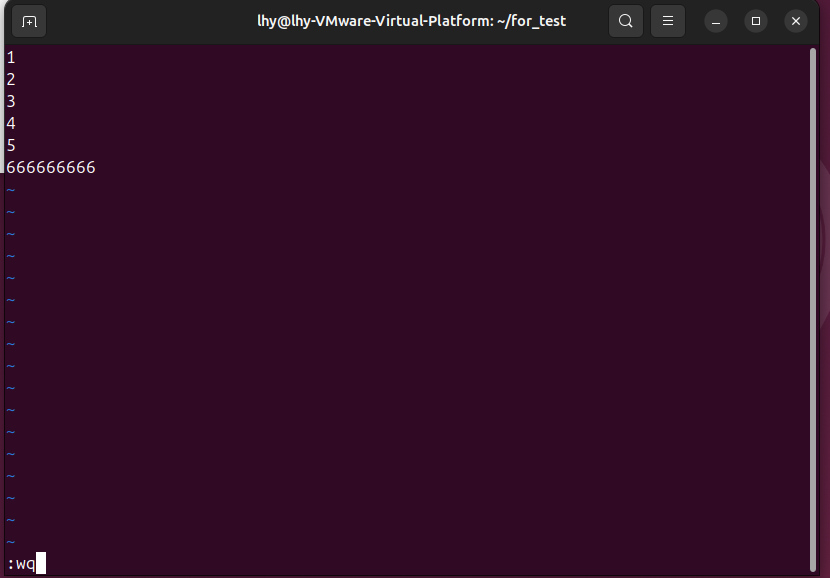
\includegraphics[width=0.8\textwidth]{lec2 (7).png}
    \caption{lec2 (7)}
    \label{fig:lec2-7}
\end{figure}
\newpage
\section*{五、实验结果}
\begin{itemize}
    \item 成功完成20个Shell与Vim操作实例;
    \item 所有脚本均能正确运行;
    \item 掌握了基本文件操作与Shell编程结构;
    \item 熟练使用Vim进行脚本编辑;
    \item 实验代码已整理并提交到https://github.com/ouc-lhy/for-lesson/tree/master/lesson2。
\end{itemize}

\section*{六、解题感悟}
通过本次实验,我系统地学习了Linux Shell和Vim的基本使用。从创建目录到编写脚本,每一步都增强了我对命令行操作的理解。Shell脚本的自动化能力令人印象深刻,而Vim作为经典编辑器,掌握其基本操作对后续学习至关重要。实验过程中遇到问题时,通过查阅资料和反复练习得以解决,提升了我的自主学习能力。今后将继续深入学习Shell高级特性,为系统开发打下坚实基础。

\section*{七、GitHub链接}
\url{https://github.com/ouc-lhy/for-lesson/tree/master/lesson2}

\end{document}